\tikzset{every picture/.style={line width=0.75pt}} %set default line width to 0.75pt        

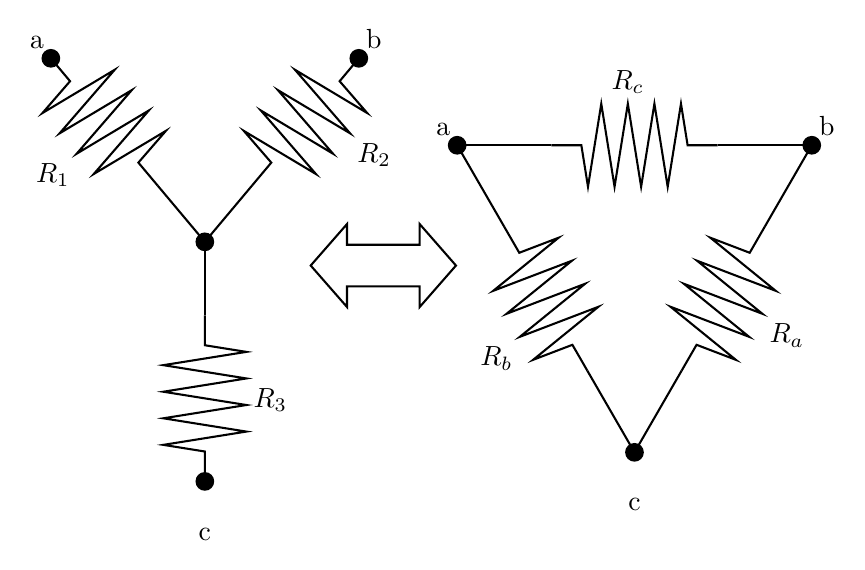
\begin{tikzpicture}[x=0.75pt,y=0.75pt,yscale=-1,xscale=1]
%uncomment if require: \path (0,420); %set diagram left start at 0, and has height of 420

%Shape: Resistor [id:dp8649111880326505] 
\draw   (219,197) -- (219,211.4) -- (239,214.6) -- (199,221) -- (239,227.4) -- (199,233.8) -- (239,240.2) -- (199,246.6) -- (239,253) -- (199,259.4) -- (219,262.6) -- (219,277) ;
%Shape: Resistor [id:dp9942934984762448] 
\draw   (241.77,134.44) -- (251.02,123.41) -- (237.76,108.11) -- (272.52,128.91) -- (245.99,98.3) -- (280.74,119.11) -- (254.22,88.5) -- (288.97,109.3) -- (262.44,78.69) -- (297.2,99.5) -- (283.94,84.19) -- (293.19,73.16) ;
%Shape: Resistor [id:dp85596491014942] 
\draw   (144.81,73.16) -- (154.06,84.19) -- (140.8,99.5) -- (175.56,78.69) -- (149.03,109.3) -- (183.78,88.5) -- (157.26,119.11) -- (192.01,98.3) -- (165.48,128.91) -- (200.24,108.11) -- (186.98,123.41) -- (196.23,134.44) ;
%Straight Lines [id:da23101519075185095] 
\draw    (219,161.58) -- (219,197) ;
%Straight Lines [id:da3890276784519242] 
\draw    (219,161.58) -- (196.23,134.44) ;
%Straight Lines [id:da7445936080781037] 
\draw    (219,161.58) -- (241.77,134.44) ;
%Shape: Circle [id:dp8383610920721991] 
\draw  [fill={rgb, 255:red, 0; green, 0; blue, 0 }  ,fill opacity=1 ] (215,161.58) .. controls (215,159.37) and (216.79,157.58) .. (219,157.58) .. controls (221.21,157.58) and (223,159.37) .. (223,161.58) .. controls (223,163.79) and (221.21,165.58) .. (219,165.58) .. controls (216.79,165.58) and (215,163.79) .. (215,161.58) -- cycle ;
%Shape: Circle [id:dp09797149394585802] 
\draw  [fill={rgb, 255:red, 0; green, 0; blue, 0 }  ,fill opacity=1 ] (289.19,73.16) .. controls (289.19,70.95) and (290.98,69.16) .. (293.19,69.16) .. controls (295.4,69.16) and (297.19,70.95) .. (297.19,73.16) .. controls (297.19,75.37) and (295.4,77.16) .. (293.19,77.16) .. controls (290.98,77.16) and (289.19,75.37) .. (289.19,73.16) -- cycle ;
%Shape: Circle [id:dp7483012020928743] 
\draw  [fill={rgb, 255:red, 0; green, 0; blue, 0 }  ,fill opacity=1 ] (140.81,73.16) .. controls (140.81,70.95) and (142.6,69.16) .. (144.81,69.16) .. controls (147.02,69.16) and (148.81,70.95) .. (148.81,73.16) .. controls (148.81,75.37) and (147.02,77.16) .. (144.81,77.16) .. controls (142.6,77.16) and (140.81,75.37) .. (140.81,73.16) -- cycle ;
%Shape: Circle [id:dp03389973177254291] 
\draw  [fill={rgb, 255:red, 0; green, 0; blue, 0 }  ,fill opacity=1 ] (215,277) .. controls (215,274.79) and (216.79,273) .. (219,273) .. controls (221.21,273) and (223,274.79) .. (223,277) .. controls (223,279.21) and (221.21,281) .. (219,281) .. controls (216.79,281) and (215,279.21) .. (215,277) -- cycle ;
%Shape: Resistor [id:dp7459678467673858] 
\draw   (386,115.05) -- (400.4,115.05) -- (403.6,135.05) -- (410,95.05) -- (416.4,135.05) -- (422.8,95.05) -- (429.2,135.05) -- (435.6,95.05) -- (442,135.05) -- (448.4,95.05) -- (451.6,115.05) -- (466,115.05) ;
%Shape: Resistor [id:dp8943386559820388] 
\draw   (448.71,223.66) -- (455.91,211.19) -- (474.83,218.42) -- (443.39,192.88) -- (481.23,207.34) -- (449.79,181.79) -- (487.63,196.25) -- (456.19,170.71) -- (494.03,185.17) -- (462.59,159.62) -- (481.51,166.85) -- (488.71,154.38) ;
%Straight Lines [id:da980522130958174] 
\draw    (386,115.05) -- (340.58,115.05) ;
%Straight Lines [id:da25013706782614387] 
\draw    (511.42,115.05) -- (466,115.05) ;
%Straight Lines [id:da024405235938776526] 
\draw    (511.42,115.05) -- (488.71,154.38) ;
%Straight Lines [id:da41196160100547097] 
\draw    (448.71,223.66) -- (426,263) ;
%Shape: Resistor [id:dp8933369509641274] 
\draw   (363.29,154.38) -- (370.49,166.85) -- (389.41,159.62) -- (357.97,185.17) -- (395.81,170.71) -- (364.37,196.25) -- (402.21,181.79) -- (370.77,207.34) -- (408.61,192.88) -- (377.17,218.42) -- (396.09,211.19) -- (403.29,223.66) ;
%Straight Lines [id:da14103113154035296] 
\draw    (426,263) -- (403.29,223.66) ;
%Straight Lines [id:da012997480095768843] 
\draw    (363.29,154.38) -- (340.58,115.05) ;
%Shape: Circle [id:dp5583976916907458] 
\draw  [fill={rgb, 255:red, 0; green, 0; blue, 0 }  ,fill opacity=1 ] (336.58,115.05) .. controls (336.58,117.26) and (338.37,119.05) .. (340.58,119.05) .. controls (342.79,119.05) and (344.58,117.26) .. (344.58,115.05) .. controls (344.58,112.84) and (342.79,111.05) .. (340.58,111.05) .. controls (338.37,111.05) and (336.58,112.84) .. (336.58,115.05) -- cycle ;
%Shape: Circle [id:dp044013820240165646] 
\draw  [fill={rgb, 255:red, 0; green, 0; blue, 0 }  ,fill opacity=1 ] (422,263) .. controls (422,265.21) and (423.79,267) .. (426,267) .. controls (428.21,267) and (430,265.21) .. (430,263) .. controls (430,260.79) and (428.21,259) .. (426,259) .. controls (423.79,259) and (422,260.79) .. (422,263) -- cycle ;
%Shape: Circle [id:dp9756959473863265] 
\draw  [fill={rgb, 255:red, 0; green, 0; blue, 0 }  ,fill opacity=1 ] (507.42,115.05) .. controls (507.42,117.26) and (509.21,119.05) .. (511.42,119.05) .. controls (513.63,119.05) and (515.42,117.26) .. (515.42,115.05) .. controls (515.42,112.84) and (513.63,111.05) .. (511.42,111.05) .. controls (509.21,111.05) and (507.42,112.84) .. (507.42,115.05) -- cycle ;
%Left Right Arrow [id:dp6518423274771699] 
\draw   (270,173) -- (287.5,153) -- (287.5,163) -- (322.5,163) -- (322.5,153) -- (340,173) -- (322.5,193) -- (322.5,183) -- (287.5,183) -- (287.5,193) -- cycle ;

% Text Node
\draw (142.81,70.16) node [anchor=south east] [inner sep=0.75pt]   [align=left] {a};
% Text Node
\draw (295.19,70.16) node [anchor=south west] [inner sep=0.75pt]   [align=left] {b};
% Text Node
\draw (219,298) node [anchor=north] [inner sep=0.75pt]   [align=left] {c};
% Text Node
\draw (489.63,199.65) node [anchor=north west][inner sep=0.75pt]    {$R_{a}$};
% Text Node
\draw (368.77,210.74) node [anchor=north east] [inner sep=0.75pt]    {$R_{b}$};
% Text Node
\draw (422.8,91.65) node [anchor=south] [inner sep=0.75pt]    {$R_{c}$};
% Text Node
\draw (338.58,112.05) node [anchor=south east] [inner sep=0.75pt]   [align=left] {a};
% Text Node
\draw (513.42,112.05) node [anchor=south west] [inner sep=0.75pt]   [align=left] {b};
% Text Node
\draw (426,284) node [anchor=north] [inner sep=0.75pt]   [align=left] {c};
% Text Node
\draw (155.26,122.51) node [anchor=north east] [inner sep=0.75pt]    {$R_{1}$};
% Text Node
\draw (290.97,112.7) node [anchor=north west][inner sep=0.75pt]    {$R_{2}$};
% Text Node
\draw (241,230.8) node [anchor=north west][inner sep=0.75pt]    {$R_{3}$};


\end{tikzpicture}
